\documentclass[11pt]{article}
\usepackage[sort]{natbib}
\usepackage{bm,amsmath,bbm,amsfonts,nicefrac,latexsym,amsmath,amsfonts,amsbsy,amscd,amsxtra,amsgen,amsopn,bbm,amsthm,amssymb,graphicx}
\usepackage{fancyhdr}
\usepackage[margin=1.0in]{geometry}
\bibliographystyle{plainnat}

\title{Improvement of forest carbon balance model DALEC2 for flux site Alice Holt using four-dimensional variational data assimilation.}
\author{Ewan Pinnington}

\newtheorem{theorem}{Theorem}[section]
\newtheorem*{defn}{Definition}


\begin{document}

\maketitle

\section{Introdution}

Four-dimensional variational data assimilation (4D-Var) has been used extensively in numerical weather prediction to improve forecasts. Currently efforts to use variational assimilation with carbon balance models have been limited, with sequential and Markov Chain Monte Carlo methods being more prevalent. In this report we will paramterize a model of forest carbon balance (DALEC2) using a 4D-Var scheme in order to produce better forecasts of forest carbon balance. We will use data from the research site at Alice Holt forest run by Forest Research.  

\section{Methods}

\subsection{4D-Var}

In 4D-Var we aim to maximise the probability of our initial state $\textbf{x}_0$ given a set of observations $\textbf{y}$, $P(\textbf{x}_0|\textbf{y})$, over some time window, $N$. $P(\textbf{x}_0|\textbf{y})$ is maximised by minimising a cost function $J(\textbf{x})$ derived from Bayes Theorem \citep{lewis2006dynamic}. The cost function is given as,

\begin{equation}
J(\textbf{x}_0) = \frac{1}{2}(\textbf{x}_0-\textbf{x}_b)^{T}\textbf{B}^{-1}(\textbf{x}_0-\textbf{x}_b)+\frac{1}{2}\sum_{i=0}^{N}(\textbf{y}_i-h_i(\textbf{x}_i))^{T}\textbf{R}_{i}^{-1}(\textbf{y}_i-h_i(\textbf{x}_i)),
\end{equation}

where $\textbf{x}_b$ is our background and acts as our initial guess to our state $\textbf{x}_0$, $\textbf{B}$ is the background error covariance matrix and quantifies our knowledge of the error in our background, $h_i$ is our observation operator at time $t_i$ and maps our state vector evolved by our nonlinear model ($m_{0\rightarrow i}(\mathbf{x}_{0})=\textbf{x}_i$) to the observations at this time ($\textbf{y}_i$) and $\textbf{R}_i$ is the observation error covariance matrix at time $t_i$ and represents our knowledge of the uncertainty in the observations. The state that minimises the cost function is called the analysis and is denoted as $\textbf{x}_a$, this state is found using a minimisation routine that takes the cost function, our initial guess ($\textbf{x}_b$) and also the gradient of the cost function defined as,

\begin{equation}
\nabla J(\textbf{x}_0) = \textbf{B}^{-1}(\textbf{x}_0-\textbf{x}_b)-\sum_{i=0}^{N}\textbf{M}_{i,0}^{T}\textbf{H}_i^{T}\textbf{R}_{i}^{-1}(\textbf{y}_i-h_i(\textbf{x}_i)),
\end{equation}

where $\textbf{H}_i = \frac{\partial h_i(\textbf{x}_i)}{\partial\textbf{x}_i}$ is our linearized observation operator and $\mathbf{M}_{i,0}=\mathbf{M}_{i-1}\mathbf{M}_{i-2}\cdots\mathbf{M}_0$ is our tangent linear model with $\mathbf{M}_i=\frac{\partial m_{i}(\textbf{x}_{i})}{\partial \textbf{x}_{i}}$. We can rewrite the cost function and its gradient to avoid the sum notation as,

\begin{equation}
J(\textbf{x}_0) = \frac{1}{2}(\textbf{x}_0-\textbf{x}_b)^{T}\textbf{B}^{-1}(\textbf{x}_0-\textbf{x}_b)+\frac{1}{2}(\hat{\textbf{y}}-\hat{h}(\textbf{x}_0))^{T}\hat{\textbf{R}}^{-1}(\hat{\textbf{y}}-\hat{h}(\textbf{x}_0)) \label{costfn}
\end{equation}
and
\begin{equation}
\nabla J(\textbf{x}_0) = \textbf{B}^{-1}(\textbf{x}_0-\textbf{x}_b)-\hat{\mathbf{H}}^{T}\hat{\textbf{R}}^{-1}(\hat{\textbf{y}}-\hat{h}(\textbf{x}_0)), \label{gradcostfn}
\end{equation}
where,
\begin{equation}
\hat{\textbf{y}}=
\begin{pmatrix}
\textbf{y}_0 \\
\textbf{y}_1\\
\vdots \\
\textbf{y}_N
\end{pmatrix},
\hspace{1mm}
\hat{h}(\textbf{x}_0)=
\begin{pmatrix}
h_0(\textbf{x}_0) \\
h_1(m_{0\rightarrow 1}(\mathbf{x}_{0}))\\
\vdots \\
h_N(m_{0\rightarrow N}(\mathbf{x}_{0}))
\end{pmatrix},
\hspace{1mm}
\hat{\mathbf{R}}=
\begin{pmatrix}
\mathbf{R}_0 & 0 & 0 & 0 \\
0 & \mathbf{R}_1 & 0 & 0 \\
0 & 0 & \ddots & 0 \\
0 & 0 & 0 & \mathbf{R}_N
\end{pmatrix}
\hspace{1mm} \text{and} \hspace{3mm}
\hat{\mathbf{H}}=
\begin{pmatrix}
\mathbf{H}_0 \\
\mathbf{H}_1\mathbf{M}_0\\
\vdots \\
\mathbf{H}_N\mathbf{M}_{N,0}
\end{pmatrix}.
\end{equation}


\subsection{The DALEC2 model}

The DALEC2 model is a simple process-based model describing the carbon balance of a forest ecosystem \citep{Bloom2014} and is the new version of the original DALEC \citep{williams2005improved}. The model is constructed of six carbon pools (labile ($C_{lab}$), foliage ($C_f$), fine roots ($C_r$), woody stems and coarse roots ($C_w$), fresh leaf and fine root litter ($C_l$) and soil organic matter and coarse woody debris ($C_s$)) linked via fluxes. The aggregated canopy model (ACM) \citep{williams1997predicting} is used to calculate daily gross primary production ($GPP$) of the forest, taking meteorological driving data and the site's leaf area index (a function of $C_f$) as arguments.   

\begin{figure}[ht]
    \centering
    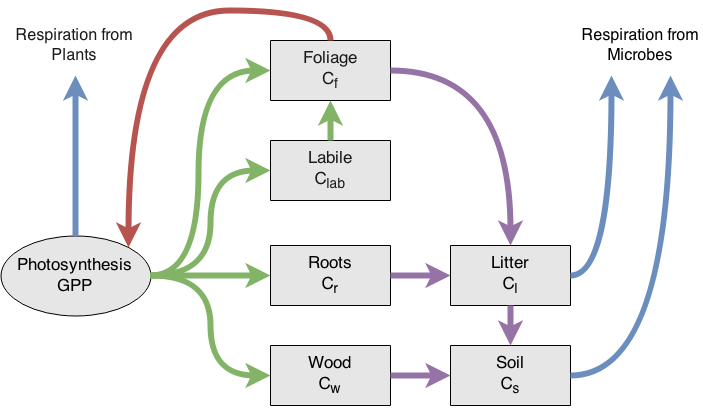
\includegraphics[width=0.5\textwidth]{Dalecdiagram.png}
    \caption{Representation of the fluxes in the DALEC2 carbon balance model. Green arrows represent C allocation, purple arrows represent litter fall and decomposition fluxes, blue arrows represent respiration fluxes and the red arrow represents the feedback of foliar carbon to the $GPP$ function.}
    \label{fig:DALEC_mod}
\end{figure}

The model equations for the carbon pools at day $t+1$ are as follows:

\begin{align}
GPP^{t} &= ACM(C_f^{t}, c_{lma}, c_{eff}, \Psi) \label{GPP}
\\C_{lab}^{t+1}&=(1-\Phi _{on})C_{lab}^{t}+(1-f_{auto})(1-f_{fol})f_{lab}GPP^{t}, \label{daleclab}
\\C_f^{t+1}&=(1-\Phi_{off})C_f^{t}+\Phi_{on}C_{lab}^{t}+(1-f_{auto})f_{fol}GPP^{t}, \label{dalec1}
\\C_r^{t+1}&=(1-\theta_{roo})C_r^{t}+(1-f_{auto})(1-f_{fol})(1-f_{lab})f_{roo}GPP^{t}, 
\\C_w^{t+1}&=(1-\theta_{woo})C_w^{t}+(1-f_{auto})(1-f_{fol})(1-f_{lab})(1-f_{roo})GPP^{t}, 
\\C_l^{t+1}&=(1-(\theta_{lit}+\theta_{min})e^{\Theta T^{t}})C_l^{t}+\theta_{roo}C_r^{t}+\Phi_{off}C_f^{t}, 
\\C_s^{t+1}&=(1-\theta_{som}e^{\Theta T^{t}})C_s^{t}+\theta_{woo}C_w^{t}+\theta_{min}e^{\Theta T^{t}}C_l^{t}, \label{dalec5}
\end{align}

where $T^{t}$ is the daily mean temperature, $\Psi$ represents the meteorological driving data used in the $GPP$ function and $\Phi_{on} / \Phi_{off}$ are functions controlling leaf on and leaf off. The model parameters used in equations \ref{GPP} to \ref{dalec5} and the equations used to calculate $GPP$, $\Phi_{on}$ and $\Phi_{off}$ are included in the appendix. The full details of this version of DALEC can be found in \cite{Bloom2014}. We now see how DALEC2 can be implemented in a 4D-Var framework.

%Forecast skill score, $SS = 1 - \frac{MSE_{forecast}}{MSE_{ref}}$, http://en.wikipedia.org/wiki/Forecast_skill

\subsection{DALEC2 4D-Var scheme}

In our DALEC2 4D-Var scheme the state vector, $\textbf{x}_0$, corresponds to the vector of the 17 model parameters and 6 initial carbon pool values defined in the appendix. We use a diagonal approximation to our background and observational error covariance matrices so that, 
$\textbf{B}=\underline{\sigma}_b^2 \textbf{I}$ and $\hat{\textbf{R}}=\underline{\sigma}_o^2 \textbf{I}$,
where $\underline{\sigma}_b$ and $\underline{\sigma}_o$ are the vectors of the background and observational standard deviations respectively, these values can be found in the appendix.

In order to find the tangent linear model (TLM) for DALEC2 we need to find the derivative of the model at each time step with respect to the 17 model parameters and the 6 carbon pools. To do this we use the AlgoPy automatic differentiation package in Python REF. For our $\textbf{x}_b$ we use a parameter set found by the University of Edinburgh using the CARbon DAta-MOdel fraMework (CARDAMOM) REF. This used Harmonized World Soil Database (HWSD) $C_{s}$ observations as initial conditions, meteorological driving data from ERA-interim and Markov chain Monte Carlo (MCMC) techniques to assimilate MODIS leaf area index (LAI) observations over a 10 year period. We now have all the tools to create our 4D-Var scheme which is implemented in Python. In sections \ref{sec:testtlm} to \ref{sec:testgrad} we will show some tests of our scheme.

\subsubsection{Test of tangent linear model} \label{sec:testtlm}

In 4D-Var we assume the tangent linear hypothesis,
\begin{equation}
m_{0\rightarrow i}(\mathbf{x}_0+\gamma \delta\mathbf{x}_0) \approx m_{0 \rightarrow i}(\mathbf{x}_0) + \mathbf{M}_{i,0}\gamma \delta\mathbf{x}_0. \label{TLH}
\end{equation}
The validity of this assumption depends on how nonlinear the model is, the length of the assimilation window and the size of the perturbation $\delta\mathbf{x}_0$. We can test this by rearranging equation~\ref{TLH} to find the relative error,
\begin{equation}
E_R=\frac{||m_{0\rightarrow i}(\mathbf{x}_0+\gamma \delta\mathbf{x}_0) - m_{0 \rightarrow i}(\mathbf{x}_0)||}{||\mathbf{M}_{i,0}\gamma\delta\mathbf{x}_0||}, \label{tlmtest}
\end{equation}
where we should have $E_R \rightarrow 0$ as $\gamma \rightarrow 0$. In figure~\ref{fig:tlm} we have plotted equation~\ref{tlmtest} for DALEC2 with a TLM evolving our state 731 days forward in time for a $5\%$ perturbation $\delta \textbf{x}_0$. Figure~\ref{fig:tlm} shows that our TLM behaves as expected for values of $\gamma$ approaching $0$.


\begin{figure}[ht]
    \centering
    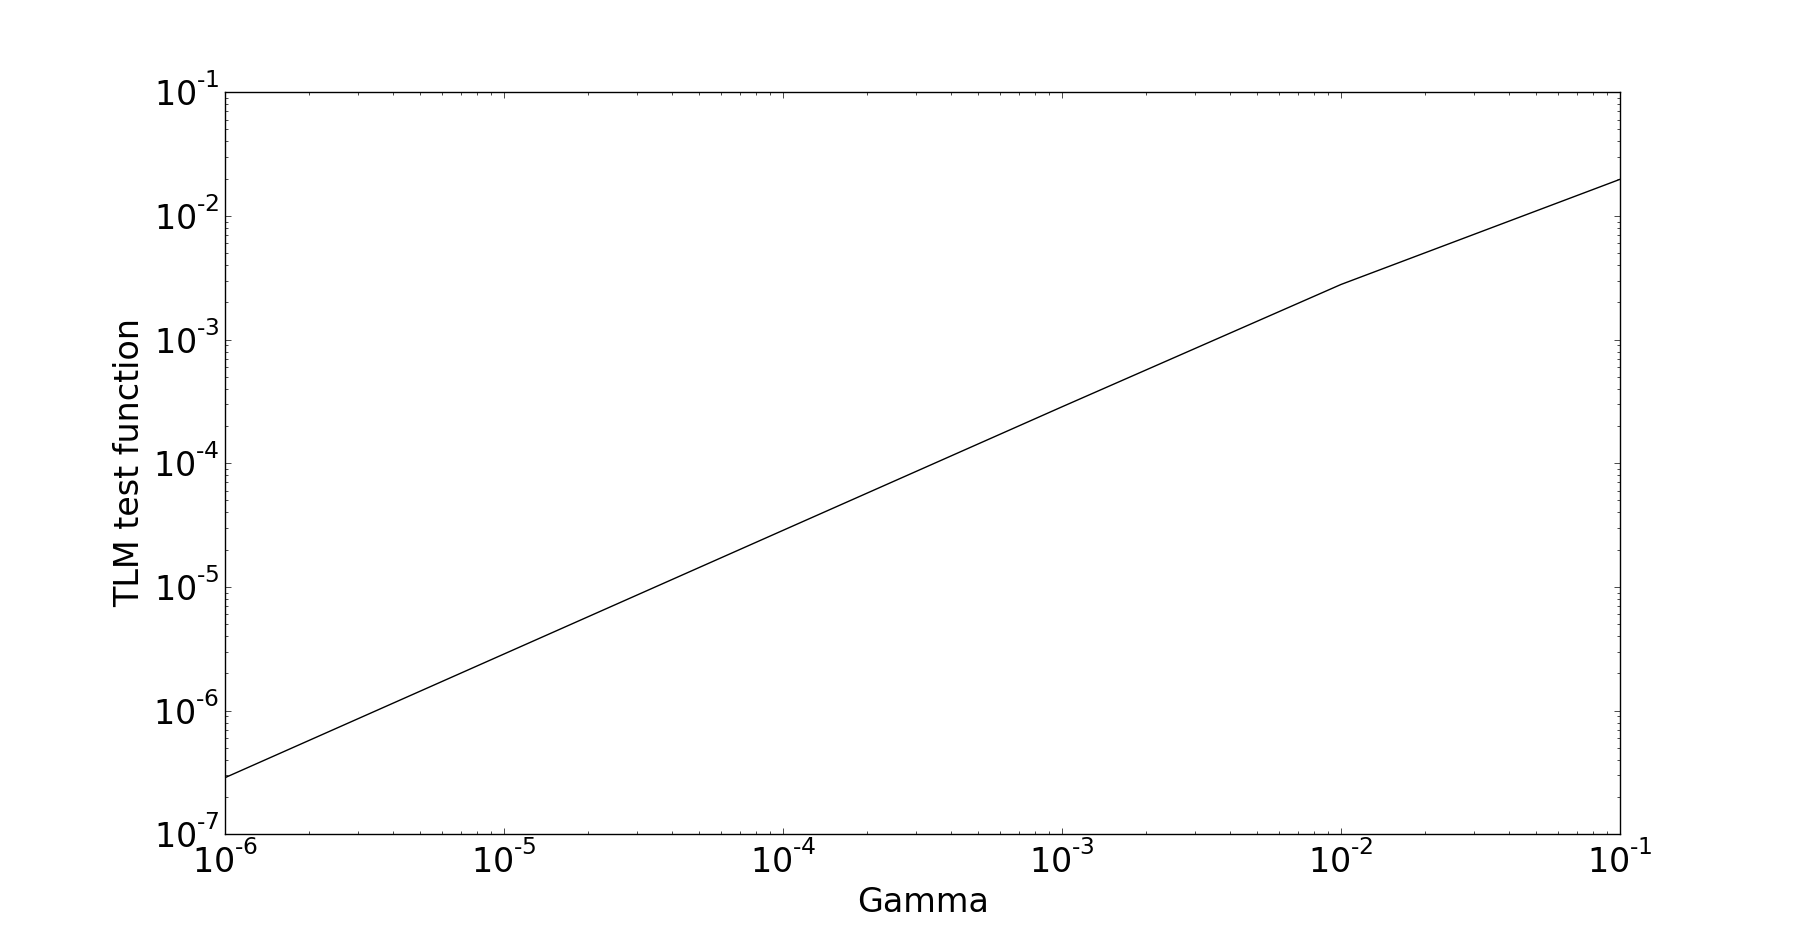
\includegraphics[width=0.8\textwidth]{testtlmer.png}
    \caption{Plot of the tangent linear model test function for DALEC2, for a TLM evolving our state 731 days forward in time and a $5\%$ perturbation, $\delta \textbf{x}_0$.}
    \label{fig:tlm}
\end{figure}

It is also useful to show how our TLM behaves over a time window to see how the error in our TLM grows as we evolve our state further forward in time. We again rearrange equation \ref{TLH} to find, 
\begin{equation}
\text{percentage error in TLM} = \begin{vmatrix} \frac{||m_{0\rightarrow i}(\mathbf{x}_0+\delta\mathbf{x}_0) - m_{0 \rightarrow i}(\mathbf{x}_0)||}{|| \mathbf{M}_{i,0}\delta\mathbf{x}_0||} - 1 \end{vmatrix} \times 100.
\end{equation}

\begin{figure}[ht]
    \centering
    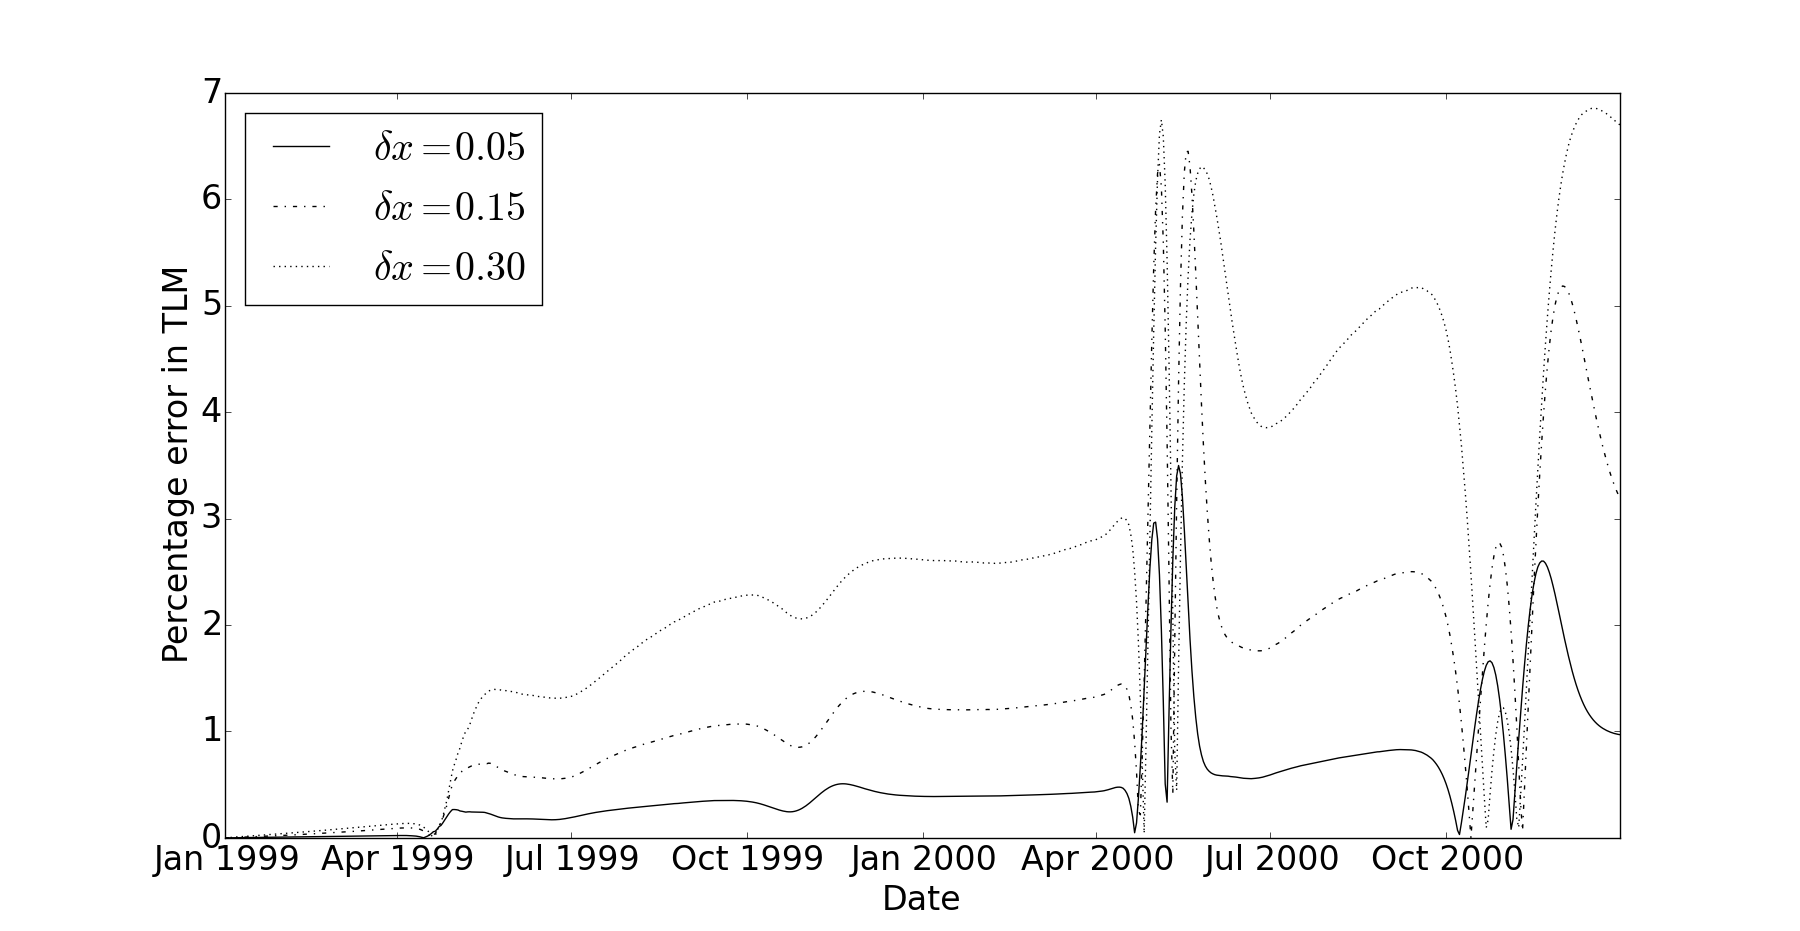
\includegraphics[width=0.8\textwidth]{tlm_error.png}
    \caption{Plot of the percentage error in our tangent linear model for DALEC2 when evolving our state forward over a period of two years with a $5\%$ perturbation, $\delta \textbf{x}_0$.}
    \label{fig:tlm_error}
\end{figure}

In figure \ref{fig:tlm_error} we can see that our TLM for DALEC2 performs very well after being run forward a year with less than a $1\%$ error. By the second year we see some peaks in our error in spring and autumn, this is where our leaf on and leaf off functions in the TLM have gone out of phase with the nonlinear DALEC2. Even at these peaks our error is still reasonable reaching a maximum at $7\%$ and then coming back to around $1\%$. 

\subsubsection{Test of adjoint model} 

For our TLM $\mathbf{M}_{i,0}$ and its adjoint $\mathbf{M}_{i,0}^{T}$ we have the identity
\begin{equation}
<\mathbf{M}_{i,0}\delta\textbf{x}_0, \mathbf{M}_{i,0}\delta\textbf{x}_0> = <\delta\textbf{x}_0, \mathbf{M}_{i,0}^{T}\mathbf{M}_{i,0}\delta\textbf{x}_0>
\end{equation}
for any inner product $<, >$ and perturbation $\delta \textbf{x}_0$. We can use this to check that our adjoint is coded correctly. 

\subsubsection{Gradient test} \label{sec:testgrad}

For our cost function $J$ and its gradient $\nabla J$ we can check that we have coded $\nabla J$ correctly using the identity,
\begin{equation}
f(\alpha)=\frac{J( \textbf{x}_0 + \alpha \textbf{h}) - J(\textbf{x}_0)}{\alpha \textbf{h}^{T} \nabla J(\textbf{x}_0)} = 1 + O(\alpha),
\end{equation}
where $\textbf{h}$ is a vector of unit length. For small values of $\alpha$ not too close to machine zero we should have $f(\alpha)$ close to 1. In figure~\ref{fig:testgradcostone} we have plotted $f(\alpha)$ for a 731 day assimilation window with $\textbf{h}=\textbf{x}_0||\textbf{x}_0||^{-1}$, we can see that $f(\alpha) \rightarrow 1$ as $\alpha \rightarrow 0$, as expected.

\begin{figure}[ht]
    \centering
    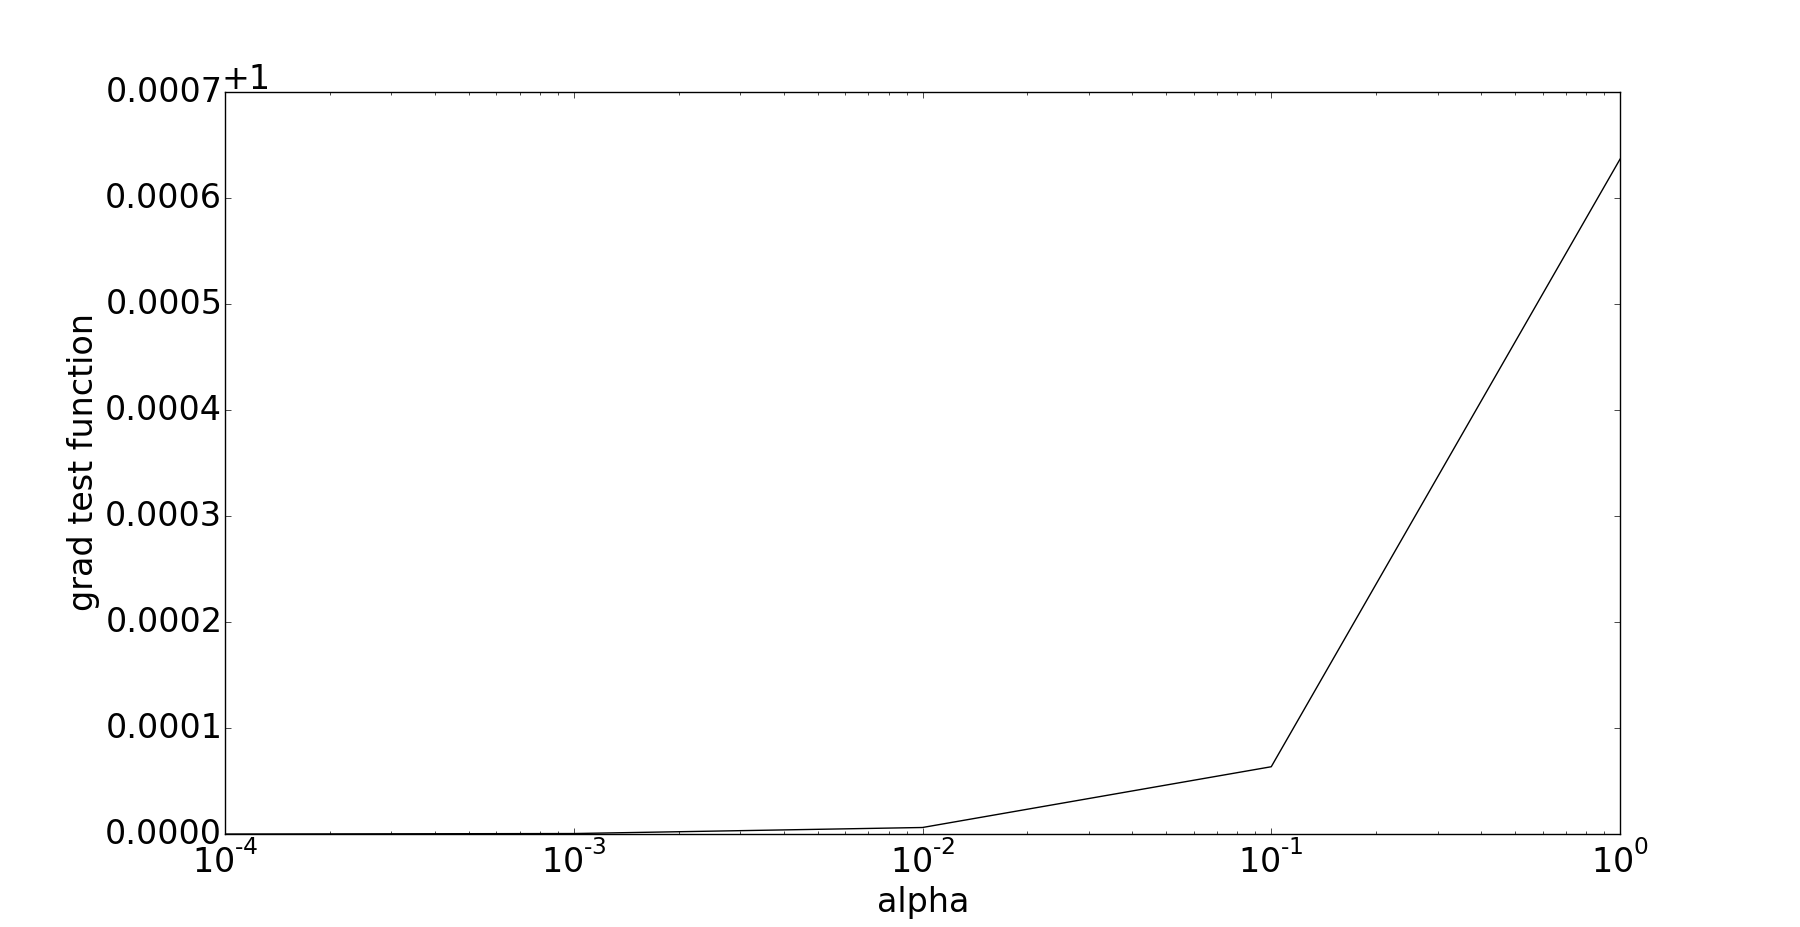
\includegraphics[width=0.8\textwidth]{gradtestone.png}
    \caption{Test of the gradient of the cost function for a 731 day assimilation window with $\textbf{h}=\textbf{x}_0||\textbf{x}_0||^{-1}$.}
    \label{fig:testgradcostone}
\end{figure}

We can also plot $|f(\alpha)-1|$, where we expect $|f(\alpha)-1| \rightarrow 0$ as $\alpha \rightarrow 0$.  In figure~\ref{fig:testgradcost} we have plotted $|f(\alpha)-1|$ for the same conditions as in figure~\ref{fig:testgradcostone}, we can see that $|f(\alpha) - 1| \rightarrow 0$ as $\alpha \rightarrow 0$, as expected (before $|f(\alpha)-1|$ gets too close to machine zero at $O(\alpha) = 10^{-5}$). This gives us confidence that the gradient of our cost function is behaving as expected.


%$\nabla J(\textbf{x}_0)||\nabla J(\textbf{x}_0)||^{-1}$. 
\begin{figure}[ht]
    \centering
    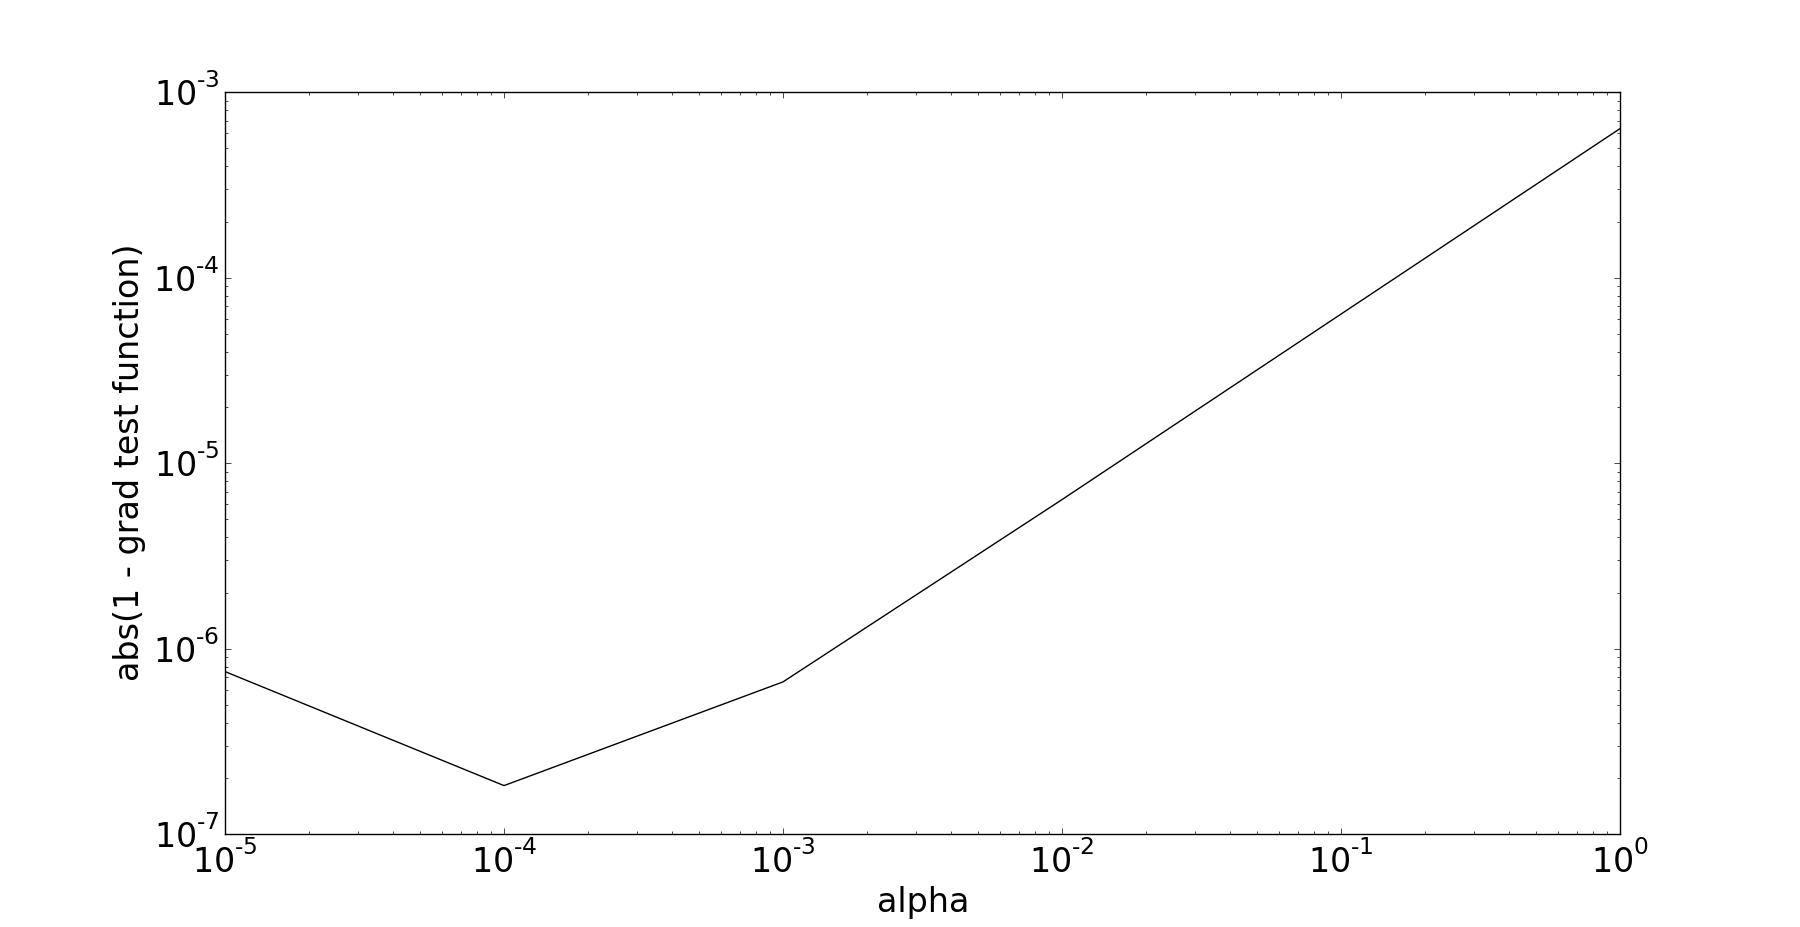
\includegraphics[width=0.8\textwidth]{testgradcost1.png}
    \caption{Test of the gradient of the cost function, $|f(\alpha) -1|$. As $\alpha \rightarrow 0$ we have $abs(1 - f(\alpha)) \rightarrow 0$ up to $O(\alpha) = 10^{-4}$ where we have gone past the precision of the computer.}
    \label{fig:testgradcost}
\end{figure}

\section{Results}


\section{Discussion}


\section{Conclusion}


\bibliography{../PhD}{}
%\bibliographystyle{plain}

\section*{Appendix}

\end{document}